\documentclass[11pt,a4paper]{report}
\usepackage[utf8]{inputenc}
\usepackage[left=2cm,right=2cm,top=2cm,bottom=2cm]{geometry}
\usepackage{color}
\definecolor{mygreen}{rgb}{0,0.6,0}
\definecolor{mygray}{rgb}{0.5,0.5,0.5}
\definecolor{mymauve}{rgb}{0.58,0,0.82}

\usepackage{amsthm}
\theoremstyle{definition}
\newtheorem{exinn}{Example}[section]
\newenvironment{example}
{\clubpenalty=10000
	\begin{exinn}%
		\mbox{}%
		{\color{blue}\leaders\hrule height .8ex depth \dimexpr-.8ex+0.8pt\relax\hfill}%
		\mbox{}\linebreak\ignorespaces}
	{\par\kern2ex\hrule\end{exinn}}

\usepackage[english]{babel}
\usepackage{amsmath}
\usepackage{amsfonts}
\usepackage{amssymb}
\usepackage{mathtools}
\usepackage{tocloft}
\usepackage{listings}
\usepackage{graphicx}
\usepackage{tikz}
\usepackage{bigints}
\usepackage{fourier}
\usepackage{fancyhdr}
\pagestyle{fancy}
\usepackage{dsfont}
\usepackage{units}
\usepackage{textcomp}
\usepackage{subcaption}
\usepackage{parskip}
\usepackage{float}
\usepackage{pdfpages}
\renewcommand{\lstlistlistingname}{Code Listings}
\renewcommand{\lstlistingname}{Code Listing}
\definecolor{gray}{gray}{0.5}
\definecolor{green}{rgb}{0,0.5,0}
\lstset{
	tabsize=4,
	rulecolor=,
	language=python,
	%basicstyle=\ttfamily\scriptsize,
	basicstyle=\footnotesize,
	upquote=true,
	numbers=left,
	numberstyle=\footnotesize,
	aboveskip={1.5\baselineskip},
	extendedchars=true,
	linewidth=\linewidth,
	breaklines=false,
	prebreak=\raisebox{0ex}[0ex][0ex]{\ensuremath{\hookleftarrow}},
	frame=single,
	columns=fullflexible,
	showtabs=false,
	showspaces=false,
	showstringspaces=false,
	identifierstyle=\ttfamily,
	keywordstyle=\color[rgb]{0,0,1},
	commentstyle=\color[rgb]{0.133,0.545,0.133},
	stringstyle=\color[rgb]{0.627,0.126,0.941},
}
\pagestyle{fancy}
\lhead{Travis Mitchell}
\rhead{Week 11}
\chead{MECH3750 - Content Summary}
\renewcommand{\headrulewidth}{0.8pt}
\renewcommand{\footrulewidth}{0.8pt}

\author{\textit{Travis Mitchell}}
\title{Lecture Content Summaries for MECH3750}
\date{Updated: 10 October, 2019}			

\makeatletter
\newcommand*{\toccontents}{\@starttoc{toc}}
\makeatother
\renewcommand{\thesection}{\thepart \arabic{section}}


\begin{document}
	\section{Elliptic PDEs}
		This week we saw the start up of a new lecturer and a focus on elliptical PDEs,
		\begin{align*}
			\partial_{xx} f + \partial_{yy} f &= 0, \\
			\nabla^2 f &= 0, \\
			\Delta f &= 0.
		\end{align*}
		Here we see that the PDE has \textbf{no} temporal derivative and thus governs \textit{steady-state} processes where the solution is influenced by the B.C. not the I.C.. As such problems are often defined by their type of boundary,
		\begin{enumerate}
			\item First boundary value problem (BVP) has Dirichlet boundaries, i.e. $f$ is fixed on the bounding surface;
			\item Second BVP has Neumann boundaries where $\partial_n f$ is defined on the bounding surface;
			\item Third BVP has Robin or mixed boundaries where $f$ may be prescribed on a portion of the boundary and $\partial_n f$ is prescribed on the remainder.
		\end{enumerate}
		\subsection{Polar coordinates}
			Often it can be useful to transform from a Cartesian type discretisation and use polar coordiantes to resolve a system. This however has to be taken into account in our governing equation,
			\begin{align*}
				x = r cos\theta \quad & \quad y=rsin\theta \\
				\implies \partial_{rr} + \partial_r f/r + \partial_{\theta \theta} f / r^2 &= 0
			\end{align*}
			The fundamental solutions in polar coordinates:
			\begin{itemize}
				\item source/sink: $f(r) = \frac{Q ln(r)}{2\pi}$
				\item vortex: $f(\theta) = \frac{\Gamma \theta}{2\pi}$
			\end{itemize}
		\subsection{Poisson equation}
			The Laplace equation is a homogeneous PDE, if we have a source term it is called Poisson's equation,
			\begin{align*}
				\partial_{xx} f + \partial_{yy} f &= S(x,y).
			\end{align*}
		\subsection{Numerical solution for the Laplace equation}
			If we consider this for a steady state heat problem, we can discretise the Laplace equation using centred finite differences,
			\begin{align*}
				\frac{T_{i+1,j} - 2T_{i,j} + T_{i-1,j}}{\Delta x^2} + \frac{T_{i,j+1} - 2T_{i,j} + T_{i,j-1}}{\Delta y^2} = 0.
			\end{align*}
			
			This gives us a two dimensional stencil which isn't typically convenient to work with so we often need to construct a single-ordinate representation of this. In doing so, we can assemble nodal equations in the form $Ax=b$, where $A$ is our coefficient matrix, $x$ is our unknown temperatures and $b$ is full of known values.\\ 
			
			To move from the $(i,j)$ mesh, one technique in Python is to use lambda functions,
			\begin{lstlisting}
X, Y = ##domain length and height
dx, dy= ##chosen discretisation
nx, ny = X/dx + 1, Y/dy + 1
m = lambda i,j: j * nx + i
			\end{lstlisting}
			
			Using this, we can then formulate our matrix,
			\begin{lstlisting}
A = scipy.sparse.lil_matrix((nx*ny,nx*ny))
for j in range(ny):
	for i in range(nx):
		p = m(i,j)
		A[p, m(i, (j-1) % ny)] = # i,j-1 stencil
		A[p, m((i-1) % nx, j)] = # i-1,j stencil
		A[p, p] = # main diagonal
		A[p, m(i, (j+1) % ny)] = # i,j+1 stencil
		A[p, m((i+1) % nx, j)] = # i+1,j stencil
A.tocsr()  #compressed sparse row matrix
			\end{lstlisting}
			
			If the problem size is small, using direct methods of solving can suffice, however, when we move to larger scale problems e.g. potentially your assignment.... Iterative methods are often favoured, Gauss-Seidel, Conjugate gradient, steepest descent etc. \\
			
			We can practice this on the question the lecture:
			\begin{figure}[h!]
				\centering
				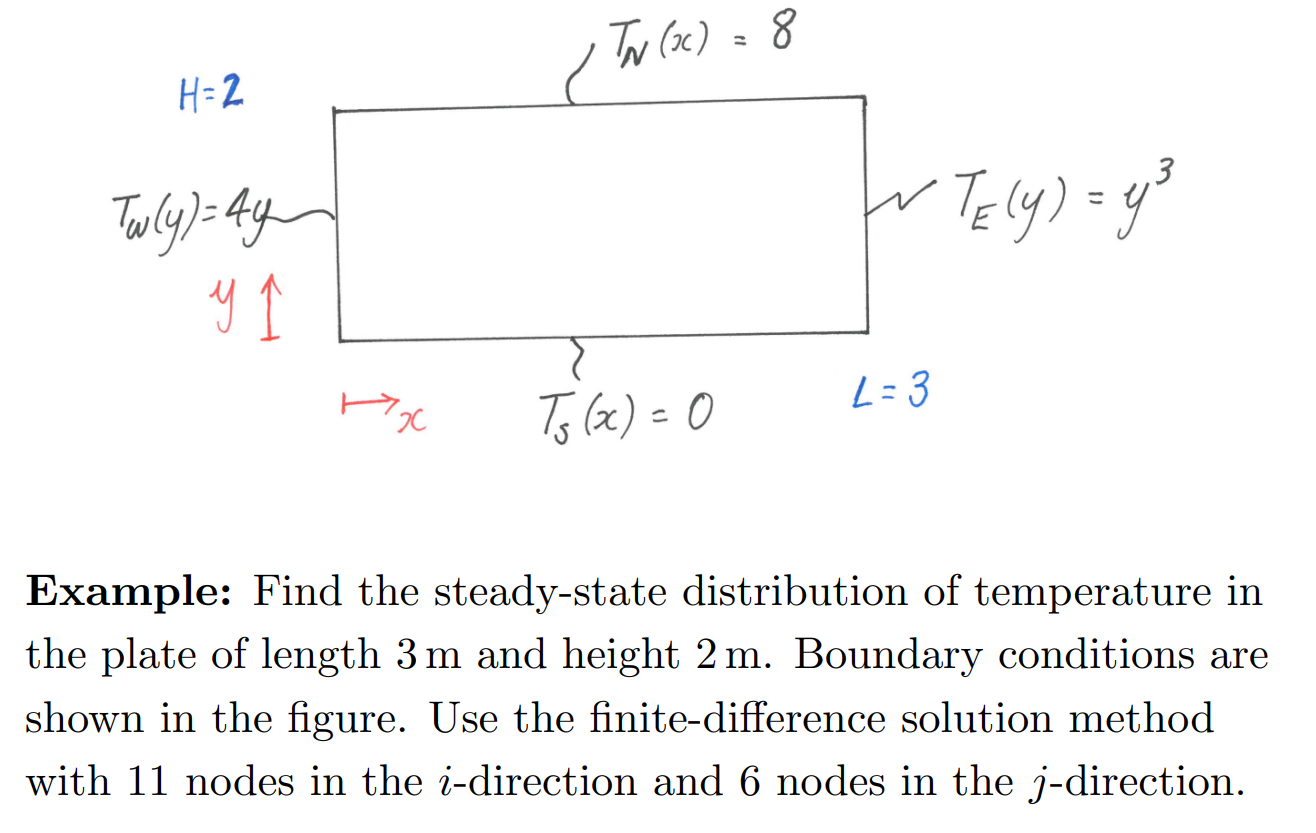
\includegraphics[width=1.0\textwidth]{work.png}
			\end{figure}
\end{document}
